\chapter{Protocol Analyzer View}

Some filters for decoding packet-oriented data provide an alternate means of visualizing the decoded traffic.

The protocol analyzer view (Fig. \ref{proto-analyzer}) displays each packet in the history as a row in a list view. The
first column is always the timestamp of the packet; remaining columns vary depending on the particular filter in
question.

Clicking on a packet pauses acquisition, loads the relevant waveform from history if the packet is not in the current
waveform, and scrolls the waveform view containing the protocol decode to the start of the packet. This allows
packet-level data to be easily correlated to physical layer waveforms.

\begin{figure}[H]
\centering
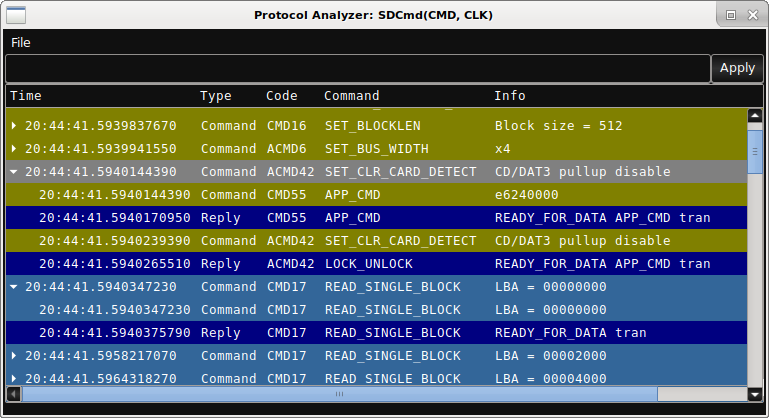
\includegraphics[width=14cm]{images/proto-analyzer.png}
\caption{Protocol analyzer view}
\label{proto-analyzer}
\end{figure}

Once closed, the protocol analyzer view may be reopened by selecting the protocol of interest from the
\menustyle{Window / Analyzer} menu.
